\begin{minipage}[t][][t]{0.6\textwidth}
    Alejandra es bióloga. En uno de sus libros se aborda el experimento del crecimiento de una población de bacterias
    respecto al crecimiento teórico reportado en literatura científica. Sin embargo, su libro se dañó y sólo se pueden apreciar
    las gráficas asociadas con expresiones algebraicas que no se ven claramente.

    \begin{parts}
        ¿Qué expresión representa el crecimiento teórico?

        \begin{oneparchoices}
            \choice $n=\dfrac{1}{2}t^2$
            \choice $n=2t$
            \choice $20=2t$
            \choice $50=\dfrac{1}{2}t^2$
        \end{oneparchoices}

        ¿Qué expresión describe el crecimiento experimental?

        \begin{oneparchoices}
            \choice $n=\dfrac{1}{2}t^2$
            \choice $n=2t$
            \choice $20=2t$
            \choice $50=\dfrac{1}{2}t^2$
        \end{oneparchoices}

        ¿En qué tiempo las expresiones de crecimiento tendrán el mismo valor?

        \begin{solutionbox}{1.2cm}

        \end{solutionbox}

        la expresión para aproximar la longitud dependiendo del tiempo, ¿es una ecuación o una identidad? ¿Por qué?

        \begin{solutionbox}{1.2cm}

        \end{solutionbox}

    \end{parts}
\end{minipage}\hfill
\begin{minipage}[t][][t]{0.35\textwidth}
    \begin{figure}[H]
        \centering
        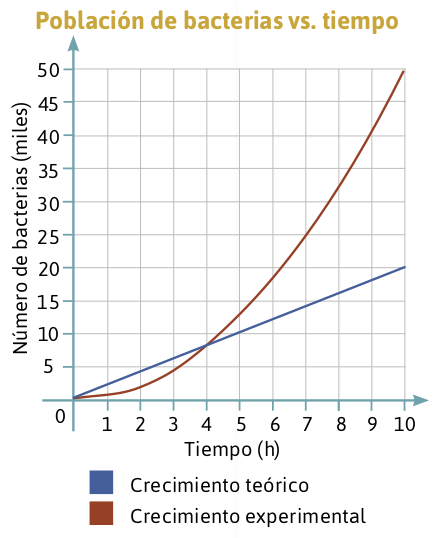
\includegraphics[width=0.9\linewidth]{../images/20230326212418}
        \caption{Población de bacterias como función del tiempo.}
        \label{fig:20230326212418}
    \end{figure}
\end{minipage}
